

\section{MECAGEN Model of Mechanic-Genetic Coupling}

  In this section, we present two mode of interaction... 
\begin{itemize}
	\item an ideal coupling mode, the proper MECAGEN model of coupling, which relates the biomechanical model introduced in Chapter 3 and the genetic and molecular regulation model introduced in Chapter 4. This coupling is what has driven the design choices behind the mechanical and genetical model. However, the principles behind the coupling will only be introduced here as, in its current state, the model has not been tested already.
	\item a simplified model of cell behavior specification, inspired by Waddington's epigenetic landscape, which bypasses the molecular and genetic regulation and allows us to test the mechanical hypotheses introduced in Chapter 3.
\end{itemize}
\begin{figure}
\begin{center}
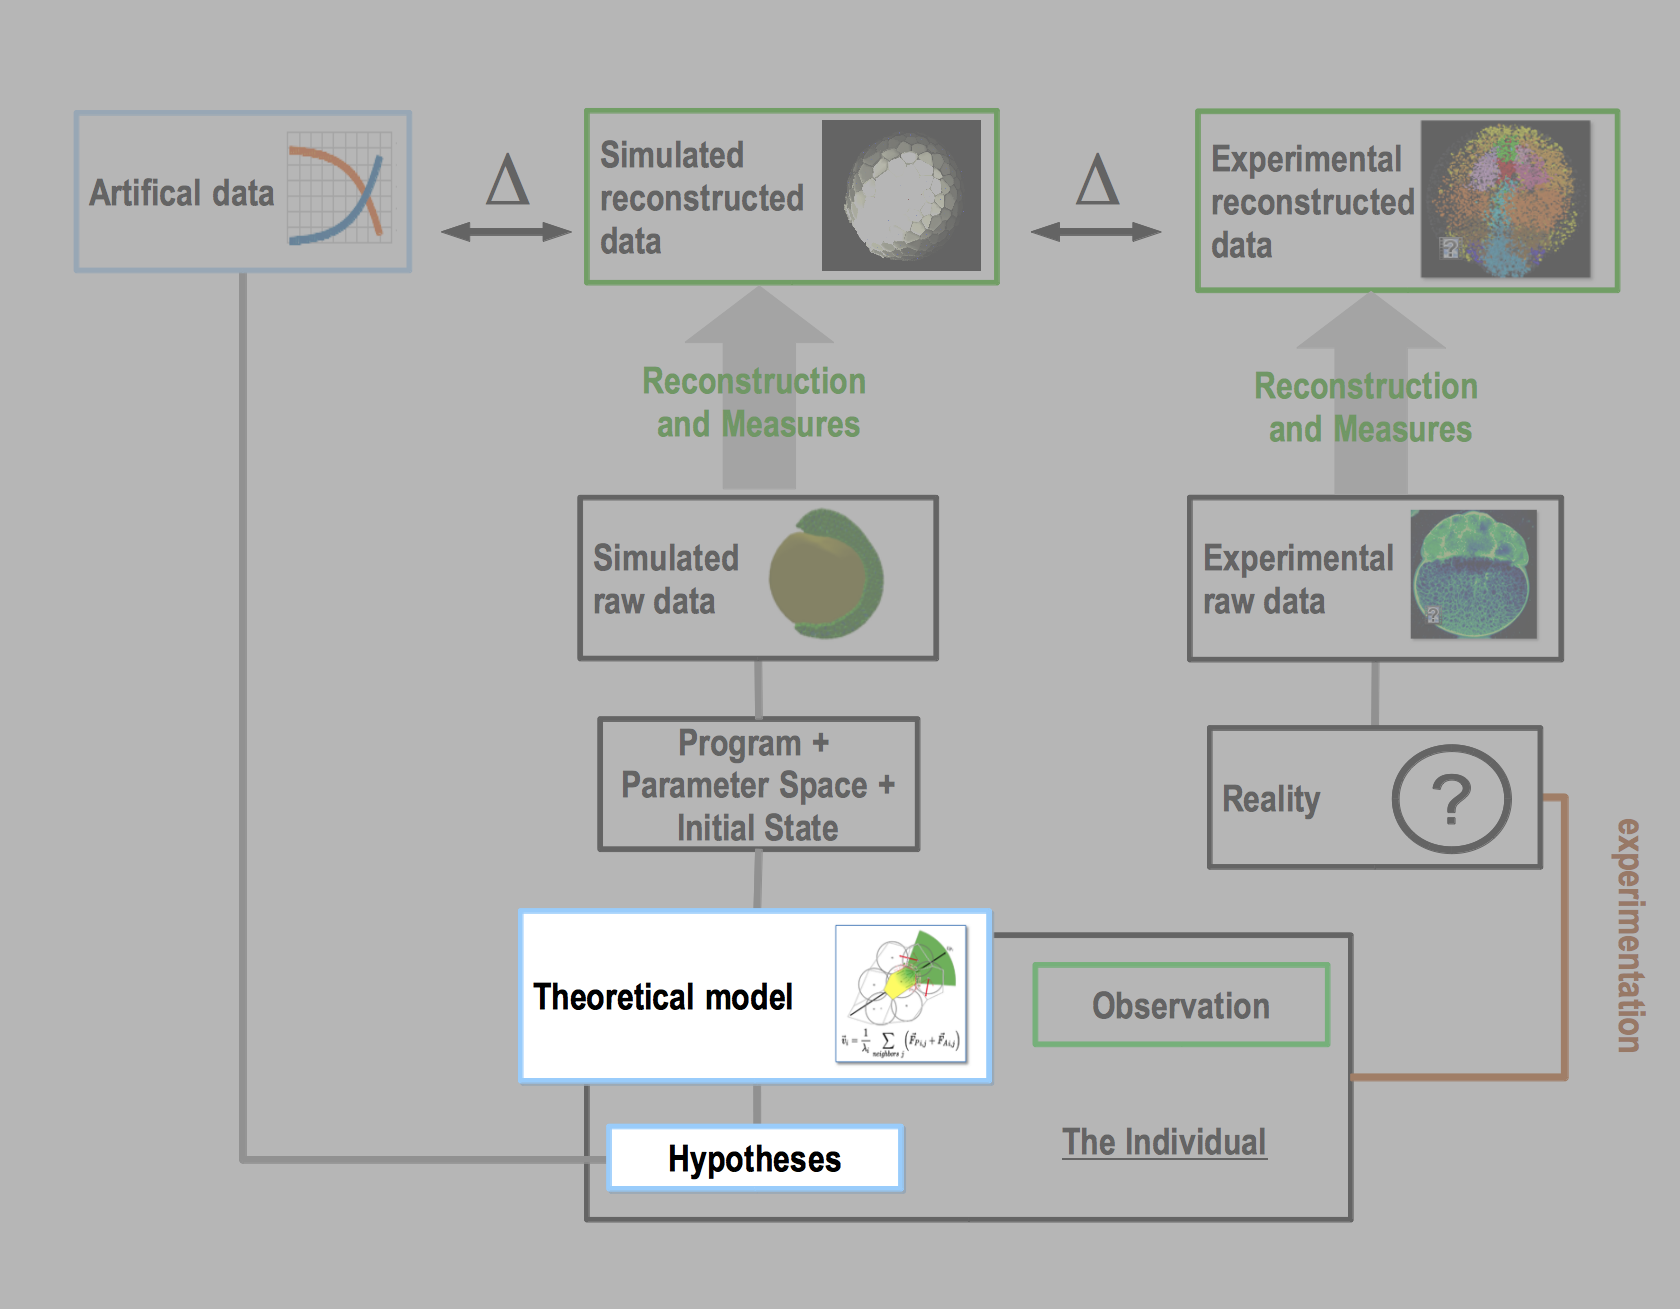
\includegraphics[width=0.75\textwidth]{../../images/experimental_science/experimental_science_cleaner_focus_theo.png}
\end{center}
\caption{\textbf{Situation of Chapter 5 in the methodological workflow.}}
\label{experimental_science_experimental_science_cleaner_focus_theo_3}
\end{figure}
%  ====================================================================== 


\subsection{Toward a Cell Behavior Ontology}
%  ====================================================================== 


  Biological system modeling requires the choice of an ontology. In our domain, the adapted ontology is a categorization of the various cell behaviors occurring during a developmental process.   Among a number of initiatives, we mention the current work of XXXX, which performs an in-depth classification of heterogeneous objects and processes involved in multi-cellular systems.   Ontologies are funded by hierarchical categories reflecting the vision of the ontology designer.    In MECAGEN, we propose to introduce a simple ontology based on the dynamical rules introduced in Chapter 3 and Chapter 4.   The objective of this ontology is establish a mapping between the genetic and molecular state of the cell and its mechanical behavior.   Ideally, all mechanical parameters must be defined by the molecular state of the cell. The spatio-temporal specification of the mechanical behavior of each cell is ruled by the dynamical outputs of its molecular and genetic regulation.    In practical terms, a predefined set of intracellular concentration levels $p_a$ is monitored, and determines the value taken by the biomechanical parameters: 
\begin{itemize}
	\item $w_{\mathrm{adh}}$, which modulates the attractive part of the \textit{relaxation} force $\vec{F}^P_{ij}$
	\item a boolean determining with the protrusive force $\vec{F}^A_{ij}$ is operating
	\item polarization axis (axes) $\vec{u}_i$
\end{itemize}

  Some cellular mechanisms are decoupled from the intracellular molecular and genetic regulation in MECAGEN: 
\begin{itemize}
	\item cell cycle length
	\item cell volume control
\end{itemize}

  Other mechanisms are not considered: 
\begin{itemize}
	\item cell death
	\item extracellular matrix
\end{itemize}
%  ---------------------------------------------------------------------- 


\subsubsection{Cell Behavior Ontology}
%  ---------------------------------------------------------------------- 


  The major dichotomy in our cell behavior ontology distinguishes the mesenchymal cell behaviors and the epithelial cell behaviors. 

  Mesenchymal cell behavior is characterized by its motility. We identify one "active" behavior for mesenchymal cells: protrusion. By protruding, mesenchymal cell are able to rearrange their neighborhood and/or migrate through it.    adhesion modulation polarization active behavior: protrusion (mono/bipolar)  

  Epithelial cell behavior is characterize by a reinforcement of lateral cellular junction. In addition, we identify two potential "active" behavior for the epithelial cells: (a)  intercalation in the sheet orthogonal to the apical-basal axis, and (b) apical constriction which allows a bending of the epithelial sheet (invagination).   apico-basal adhesion lateral adhesion specification of an apical-basal polarization axis reinforced lateral adhesion active behavior1: apico-basal contraction (torquing ) active behavior2: active intercalation in the lateral plane (only, require an additional axis).  
%  ---------------------------------------------------------------------- 


\subsubsection{Cell Adhesion}
%  ---------------------------------------------------------------------- 


  Cell adhesion is the mechanical phenomenon that is the easiest to relate to an output of the molecular and genetic regulation. The intensity of the adhesion between two neighbor cells is a function of the surface densities of adhesion molecules. Assuming that the adhesive molecules are uniformly distributed on the cell membrane and that the intracellular protein $P_a$ is the adhesive molecule in the following, we define, at the interface between two neighbor cells $i$ and $j$, the surface concentration $c_{a,i,j}$ (resp. $c_{a,j,i}$) of $P_a$ on the membrane of $i$ (resp. $j$): 

  $$ c_{a,i,j} = \frac{p_{a,i} A_{i,j}}{4 \pi {R_i}^2} $$ 

  $$ c_{a,j,i} = \frac{p_{a,j} A_{i,j}}{4 \pi {R_j}^2} $$ 

  where $p_{a,i}$ (resp. $p_{a,j}$) is the internal concentration of protein $P_a$ in cell $i$ (resp. $j$), A_{i,j} is the surface of contact between $i$ and $j$ introduced in Chapter 3 and $R_i$ (resp. $R_j$) is the radius of cell $i$ (resp. $j$). 

  We also assume that adhesive molecule bind individually at the cell-cell interface \cite{Boggon:2002da} (other modes of binding are explored in \cite{Zhang:2011ca}), the equation of the adhesion coefficient $w_{\mathrm{adh}, a, i, j}$ of the "relaxation" force $\vec{F_{ij}^P}$ induced by the adhesion molecule $P_a$ reads: 

  $$ w_{\mathrm{adh}, a} = k_{\mathrm{adh},a} c_{a,i,j} c_{a,j,i} $$ 

  where $k_{\mathrm{adh},a}$ is an adhesion constant proper to $a$. 

  Multiple adhesive molecules type may be involved in between two neighbor cells, we assume that each molecule type exerts homotypic adhesion, i.e. they bind only with their own kind. For this reason, if multiple cell adhesion molecules $P_a$ with $a=0...N_{\mathrm{adh}}$ are involved at a cell-cell interface, we sum each molecule type contribution: 

  $$ w_{\mathrm{adh}} = \sum_{a = 0}^{N_{\mathrm{adh}}} w_{\mathrm{adh},a} $$ 
%  ---------------------------------------------------------------------- 


\subsubsection{Cell Polarization}
%  ---------------------------------------------------------------------- 


  Every "active" cell behaviors exploited in MECAGEN require a polarization axis. In real cells, polarization translates into an asymmetry of the intracellular molecules. However in MECAGEN, there is no spatialization of intracellular material. We represent this asymmetry by a 3D vector passing through the center of the cell. Moreover, as the developmental process unfolds, a MECAGEN cell is potentially polarized through different polarization mechanisms. For a generic cell $i$, we denote these $N_d$ potential polarization axes $\vec{u}_{d,i}$ with $d=0...N_d\!-\!1$ and introduced an additional boolean variable $\mathbf{\Delta} = \Delta_d$, which is 1 (resp. 0) if the $\textrm{d}^{\textrm{th}}$ polarization mechanism is active (resp. not). Ideally, mesenchymal have at most one non-null $\Delta_d$ whether a mesenchymal active behavior is acting, and an epithelial cell have at least one non-null $\Delta_d$ (for the calculation of the apical-basal axis) and at most two non-null $\Delta_d$ whether an epithelial active behavior is acting. We introduce here three different modes of determination of the axis of polarization: (a) a local gradient-based mode, (b) a cell-cell contact propagation mode, and (c) a force induced mode. Additionally, a default mode (d) is activated if a polarized cell lacks any inputs for the three aforementioned mechanisms. The default mode stochastically re-orients the polarization axis until another polarization mode take over. 

  Before presenting the four modes of polarization axis specification, we explain the updating procedure of the current polarization axis of a cell. The new axis of polarization is instantaneously calculated in a simulation step, however, the cell does not immediately adopt this new axis as there is inertia between the moment the cell sense its environment and the moment the cell effectively adopt the new axis. We denote by $\vec{u}_{d,i}^{\mathrm{update}}$ the update axis of polarization. We model this damped evolution of the cell polarization as the following:  

  Je le mets en algorithme car je ne vois pas d'autre solution: 

  1. normalization step (pour Ren�, je mets cette normalization ici car je n'ai pas r�ussi à exprimer directement le vecteur d'axe de polarization $\vec{u}_{d,i}^{\mathrm{update}}$ directement normalis� dans les expressions (a) (b) (c), voir plus bas):  

  $$ \vec{u}_{d,i}^{\mathrm{update}} \leftharpoonup \frac{\vec{u}_{d,i}^{\mathrm{update}}}{\left \| \vec{u}_{d,i}^{\mathrm{update}} \right \|} $$ 

  2. update of the current polarization axis with a "forgetting" coefficient $\omega$ ($\omega \geq 0$ with $\omega = 0$ if the update is "memory-less"). 

  $$ \vec{u}_{d,i} \leftharpoonup \omega \vec{u}_{d,i} + \vec{u}_{d,i}^{\mathrm{update}} $$ 

  3. second normalization step  

  $$ \vec{u}_{d,i} \leftharpoonup \frac{\vec{u}_{d,i}}{\left \| \vec{u}_{d,i} \right \|} $$ 

  We present now the four modes of polarization: 
\begin{itemize}
	\item (a) local gradient-based mode. This mode expresses a classical vision of polarization, e.g. often used in chemotactic cell behaviors, and supposes that the cell is able to detect an asymmetry of the extracellular ligand concentration in its local vicinity. In MECAGEN, this asymmetry is determined using the abstract graph of neighborhood relationships (Section 3.2.2) and the extracellular ligand quantities $q_a$ (Section 4.2.1). This mode of axis specification is associated with a ligand type $Q_a$ and define the axis polarization ($\vec{u}_i = \vec{u}_{a,i}$) as the average of the neighborhood links weighted by a polynomial function of the difference of local ligand quantities:
\end{itemize}

  $$ \vec{u}_{d,i}^{\mathrm{update}} = \sum_{j \in \mathcal{N}^t_i} (q_{a,j} - q_{a,i})^n \vec{u}_{ij} $$ 

  where $\mathcal{N}^{t}_i$ is the list of topological neighbors of cell $i$, $q_{a,i}$ (resp. $q_{a,j}$) is the local quantity of extracellular ligand $Q_a$ around $i$ (resp. $j$), $n$ is a integer controlling the sensibility of the detection of the local asymmetry ($n$ have to be an odd number, and typically is equal to 3), and $\vec{u}_{ij}$ the unit vector pointing from $i$ to $j$. 
\begin{itemize}
	\item    (b) cell-cell contact propagation mode. This mode expresses another way of propagating  polarization axes in a cellular field. It is based on the notion that the asymmetric spatialization of intracellular material in a polarized cell translates into a surfacic asymmetry that neighbor cells can sense. Only polarized neighbors ($\Delta_d = 1$) influence their vicinity. Thus, the cell-cell contact propagation mode define the polarization axis of cell $i$ has the average of its polarized neighbors' polarization axes.  
\end{itemize}

  $$ \vec{u}_{d,i}^{\mathrm{update}} = \sum_{j \in \mathcal{N}^t_i} \Delta_{d,i} \vec{u}_{d,j} $$ 

  This mode is systematically used for the determination of the apical-basal axis in an epithelial sheet of cells. Only the lateral neighbors belonging to the topological list of neighbors $\mathcal{N}^t_i$ are considered in the sum (i.e. neighbor whose normalized neighboring link and apical-basal polarization axis forms a absolute scalar product less .25). 
\begin{itemize}
	\item    (c) force-induced mode. Recent studies unveil a novel mechanisms for the propagation of polarization axis based on the mechanical interaction \cite{Weber:2011hi}\cite{Dumortier:2012jk}. Weber et al. \cite{Weber:2011hi} demonstrates that a mechanical traction exerted at one end of a \textit{Xenopus} cell triggers the formation of protrusion in the opposite direction through a reorganization of internal keratin intermediate filaments. In MECAGEN, we idealize this mechanism by orienting the polarization axis in the direction opposite to the averaged force exerted by neighbor protruding cells.  
\end{itemize}

  $$ \vec{u}_{d,i}^{\mathrm{update}} = - \frac{1}{N_{\textrm{protrusion}}} \sum_{j \in \mathcal{N}^t_i} \vec{F}^A_{ji}  $$ 

  where $\vec{F}^A_{ji}$ is the "active" force exerted by the neighbor $j$ on $i$, and $N_{\textrm{protrusion}}$ is the number of neighbor cells exerting protrusion on j. 
\begin{itemize}
	\item (d) Default mode. As a protruding cell does not receive spatial cue allowing it to orient, they often enter a "blebbing" st. In MECAGEN, these cells receive a new polarization axis with random orientation at regular time interval (time period of generation of the random axis $T_g$) Typically, the time period is 5 minutes. Each spatial coordinate of the polarization vector is randomly generated. 
\end{itemize}

  Update of the polarization axis   Default polarization mode: random orientation Update inertia   
%  ---------------------------------------------------------------------- 


\subsubsection{Mechanotransduction Input of the GRN}
%  ---------------------------------------------------------------------- 


  Recent studies have shown that some genes are upregulated by mechanical forces exerted on the cell \cite{Desprat:2008ei}. This mechanism is among the funding principles in MECAGEN, allowing a real coupling of the mechanical domain to the molecular and genetic regulation. Practically, we add a new module to our molecular and genetic simulation platform. If the module is active, i.e. the sum of the forces exerted on the cell are above a given threshold, this module increases its target protein $P_a$ concentration by a simple equation, based on a constant production coefficient $\xi_a$ characteristic of the module.  

$$\frac{dp_a}{dt} = \xi_a$$  Cell protrusion  a. monopolaire ou bi_polaire (chapitre 3) b. intensit� de la protrusion (chapitre 3) c. protrusion target, function of cell types (chapitre 5) d. axe de polarization  protrusion -> module ((rho rac gtpase)) a set of molecule whose state determine if the cell will perform protrusive activity protrusion -> axis, monopolar, bipolar, substrate  We expect a protruding cell to be active if it orients its protrusion(s) along   protrusion -> axis, monopolar, bipolar, substrate  polarization -> eventuellement relier au module de protrusion  necessite une spatialization au niveau subcellulaire, assymetrie cytoplasmique.  par defaut random...  mode ligand mode average mode mechanotransduction both  update pas instantan�...  epithelial behaviors:  apico-basal specification  stronger lateral adhesion  additional mechanisms: apical-constriction   
%  ====================================================================== 


\subsection{Waddingtonian Timeline Specification}
%  ====================================================================== 
  Expliquer pourquoi on n'utilise pas le model complet dans la suite  

  Even if, ultimately in MECAGEN, the real causes (causing factors/inputs of the model) behind the embryo development are the molecular and genetic parameters specified by a BioTapestry GRN, we also aim at studying development through the spectrum of cell forces alone. As Odell et al. mentioned in \ref{{Odell:1981vy}}, cell forces, equivalently to "clocks, morphogens, or potentials",  are the "cause" which "explains" the "morphogenetic motion". For this goal, we decide to uncouple to coupled MECAGEN model and bypass the molecular and genetic interaction. The cell behaviors will be attributed not on the ground of the GRN outputs, but rather as the direct reading a novel parameter specification tool, called \textit{Waddingtonian landscape specification}. This tool is inspired by the famous \textit{epigenetic landscape} introduced by Waddington in "The Strategy of the Genes" \cite{Waddington:1957te}. The epigenetic landscape views the development as a dynamical system in which the cells evolve through time towards attractors represented as foldings (he called "creodes") on a hillside (Fig. \ref{Development_Review_waddington_epigenetic_nature_mod_small}). The cell fate, symbolized by a ball rolling down the hillside, falls into on or another attractor under the influence of inducing signals.  
\begin{figure}
\begin{center}
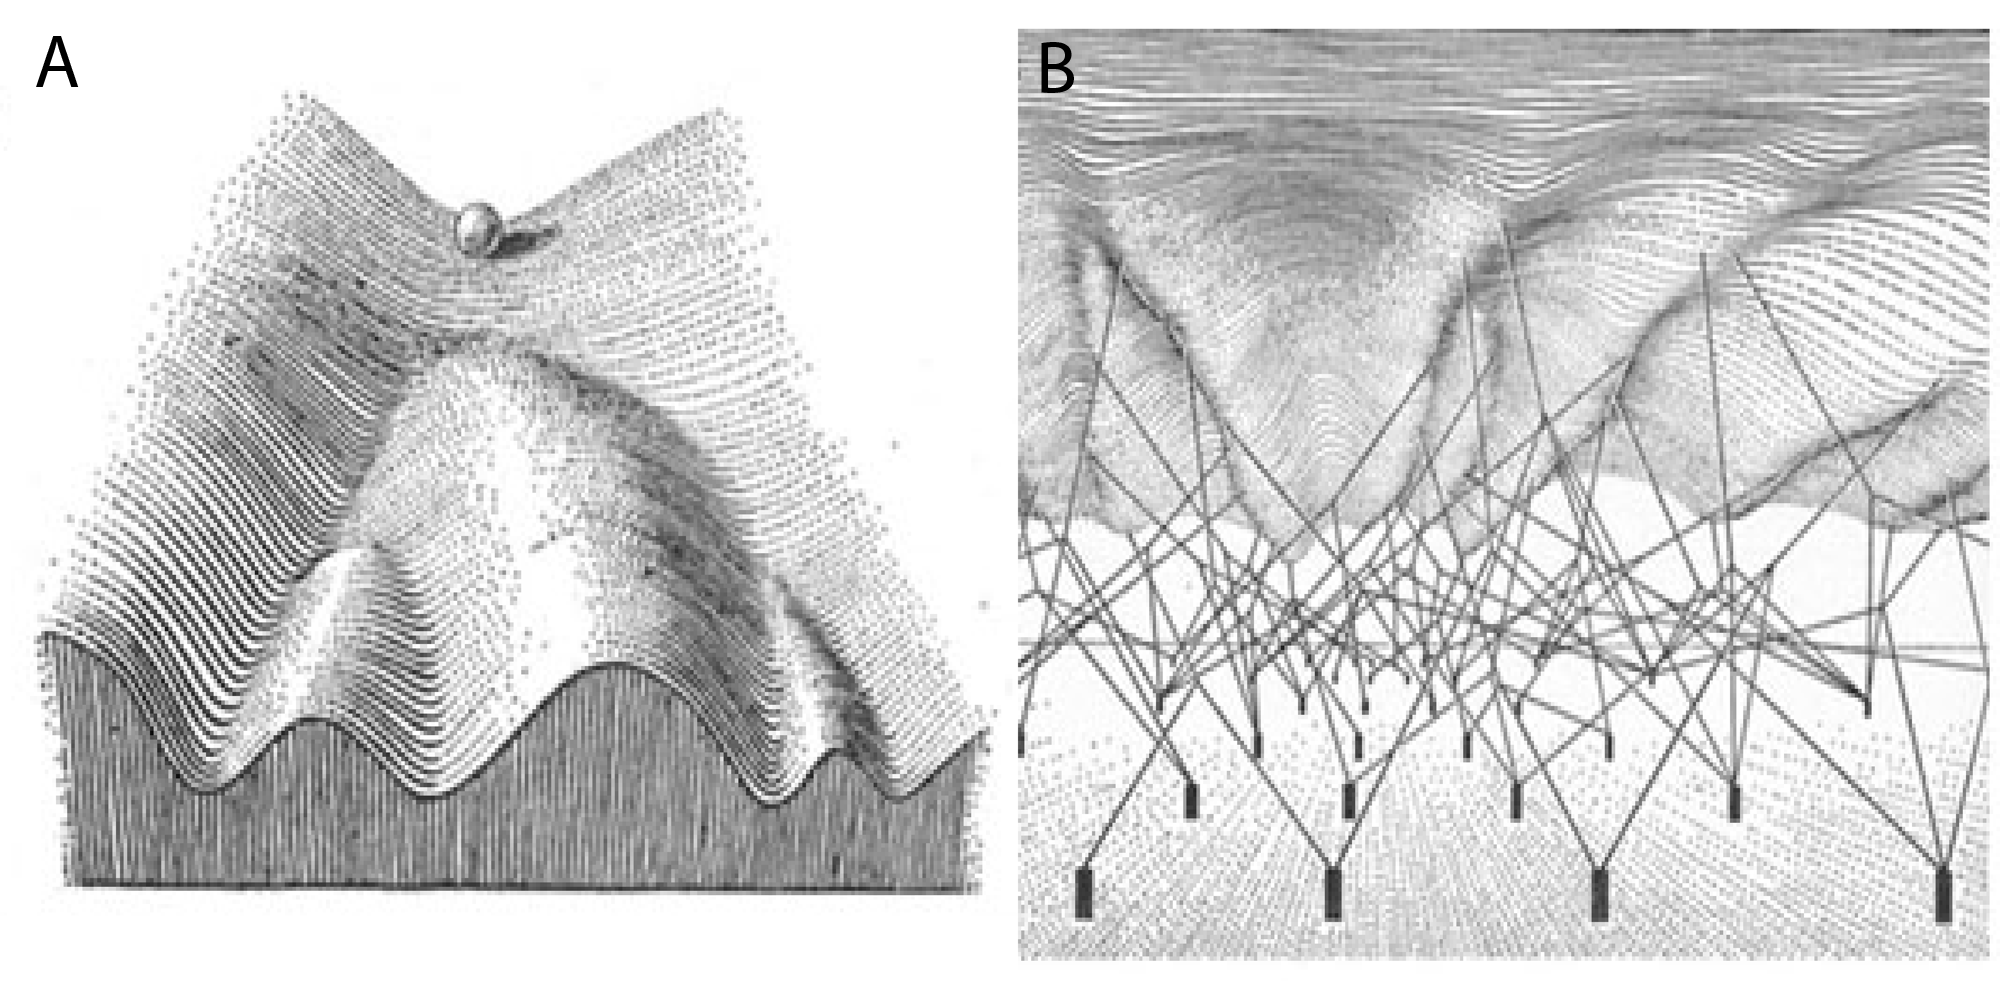
\includegraphics[width=0.8\textwidth]{../../images/Development_Review/waddington_epigenetic_nature_mod_small.png}
\end{center}
\caption{\textbf{Waddington's epigenetic landscape.} A: The ball represents a cell evolving in the epigenetic landscape. Its fate is determined by the canals in which the ball is rolling. B: A view of the landscape's behind the scene. The landscape relief is dynamically controlled by hidden wires which symbolized the gene expression and interactions. Image and legend adapted from Slack \cite{Slack:2002kg}}
\label{Development_Review_waddington_epigenetic_nature_mod_small}
\end{figure}

  In the following, we present how are specified the parameters of a Waddingtonian timeline. A specific graphical interface has been developed in this purpose. 
%  ---------------------------------------------------------------------- 


\subsubsection{Cell Types}
%  ---------------------------------------------------------------------- 


  The first step of a Waddingtonian timeline specification is to "carve the hillside" by attributing \textit{cell types} that the cell can potentially adopt during the developmental process. We define \textit{stages} which are the time point from which a bifurcation of cell type is possible. Then, we specify the conditions which will induce a cell to change its type. We call this process \textit{differentiation}. The differentiation are simply expressed by a position information-like mechanism: if a specified ligand has a local value exceeding a given threshold, the cell switch its type. The cell types are represented as a tree which expands itself through time (Fig. \ref{waddingtonian_timeline_timeline}). 
\begin{figure}
\begin{center}
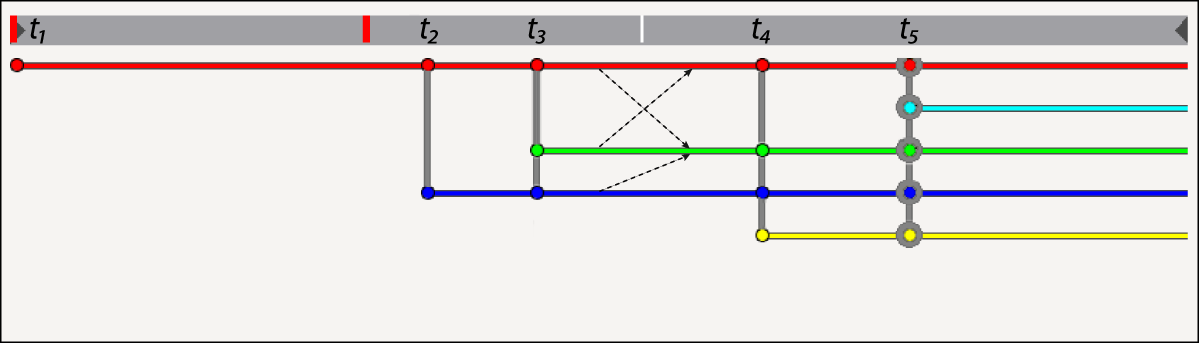
\includegraphics[width=0.8\textwidth]{../../images/MECAGEN/waddingtonian_timeline/timeline.png}
\end{center}
\caption{\textbf{Waddingtonian timeline.} The grey bar on top is the time axis, starting from the left to the right. The thin white bar is the current time step of a simulation. Thick red bars symbolize buckets from which the whole state of a simulation is recorded as the white time bar passes through it. It is a convenient way of specifying simulation snapshots. The colored bifurcating branches are the cell type that the cells can potentially take. The dots are the stages from which the simulation parameters are specified. A stage comprise all the vertical dots at a given time step, thus we can observe 5 stages in the timeline.}
\label{waddingtonian_timeline_timeline}
\end{figure}
%  ---------------------------------------------------------------------- 


\subsubsection{Ligand Sinks and Sources}
%  ---------------------------------------------------------------------- 


  Once the backbone of the waddingtonian timeline has been designed, the diffusing ligands must be specified. At each stages, we define sources and sinks for each ligands. Each cell types can secrete or absorb any ligands (Fig. \ref{waddingtonian_timeline_sources_sinks}). Additionally, spatial specification of the ligands sources are possible. External sources of ligands may also be added (e.g. in Chapter 8, the yolk egg is a source of ligand). 
\begin{figure}
\begin{center}
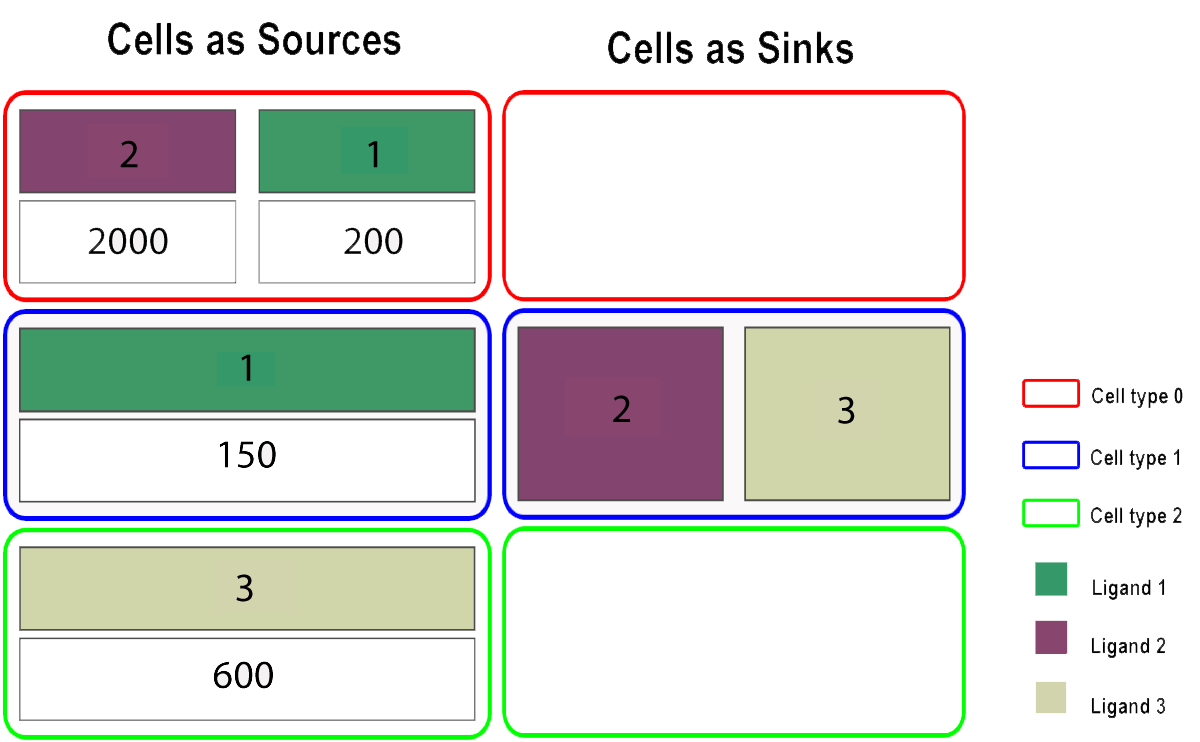
\includegraphics[width=0.7\textwidth]{../../images/MECAGEN/waddingtonian_timeline/sources_sinks.png}
\end{center}
\caption{\textbf{Ligands cells' sources and sinks specification.} Left: }
\label{waddingtonian_timeline_sources_sinks}
\end{figure}
%  ---------------------------------------------------------------------- 


\subsubsection{Passive Force's Adhesion Modulation}
%  ---------------------------------------------------------------------- 


  The adhesion coefficient $w_{\mathrm{adh}}$ of the relaxation force $\vec{F}^P$ is specified for each potential cell type's interaction (Fig. XX). 
\begin{figure}
\begin{center}
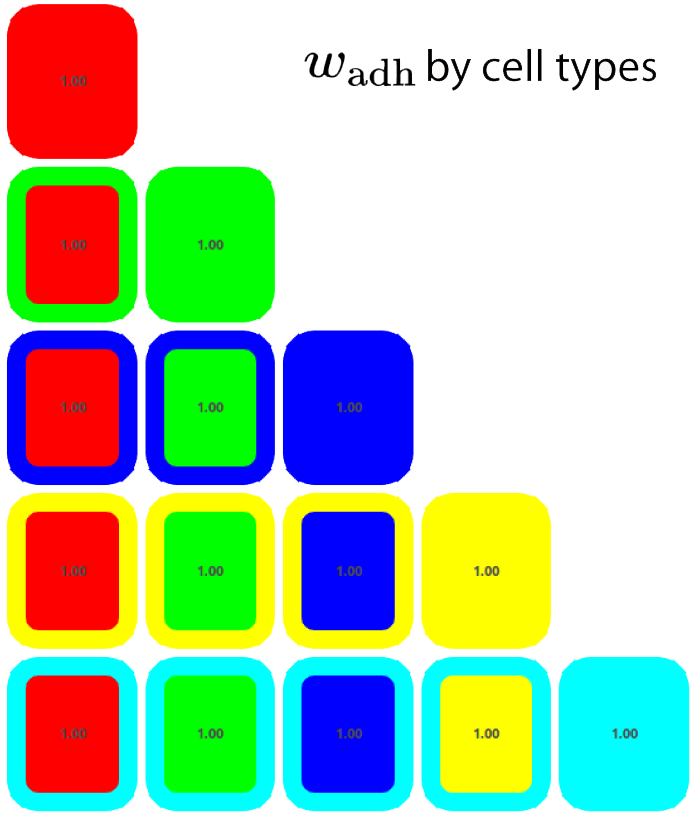
\includegraphics[width=0.4\textwidth]{../../images/MECAGEN/waddingtonian_timeline/adhesion.png}
\end{center}
\caption{\textbf{Adhesion coefficient in the Waddingtonian timeline gui.} The matrix must be symmetrical so only half of the coefficients are displayed. Cell types' color code is the same as Fig. \ref{waddingtonian_timeline_timeline}.}
\label{waddingtonian_timeline_adhesion}
\end{figure}
%  ---------------------------------------------------------------------- 


\subsubsection{Active Cell Behavior Specification}
%  ---------------------------------------------------------------------- 


  Once the ligand sources and sinks are defined, the active cell behavior are specified by adding behavioral module for a given cell type at a given stage. A protrusion module (Fig. \ref{waddingtonian_timeline_protrusion}) is associated to a cell type and gets four parameters: the target cell type on which the protrusion takes effect, the id of the axes of protrusion (axes of protrusion are calculated by the ligand mode (a) defined in Section 5.1), the intensity of the protrusive force, and an boolean of value 0 (resp. 1) if the cell is monopolar (resp. bipolar). 
\begin{figure}
\begin{center}
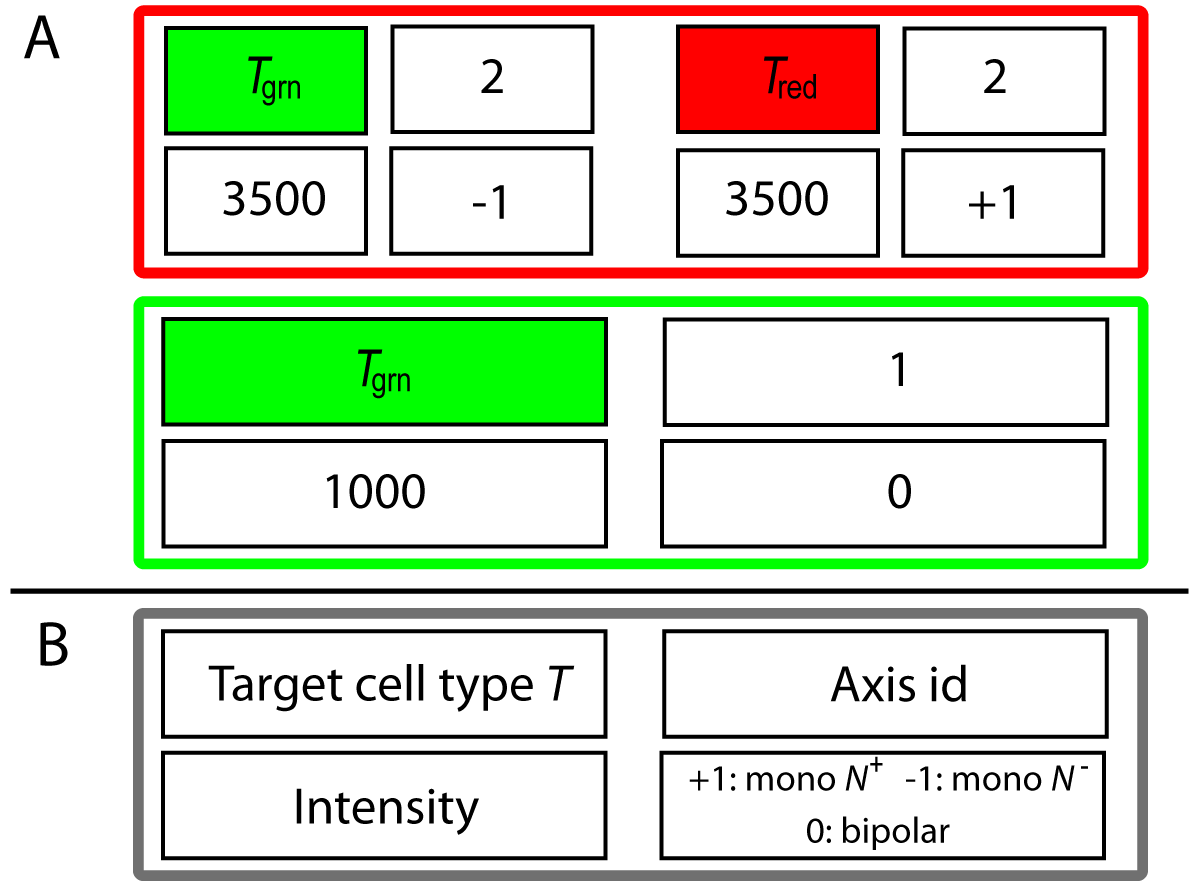
\includegraphics[width=0.4\textwidth]{../../images/MECAGEN/waddingtonian_timeline/protrusion2.png}
\end{center}
\caption{\textbf{Protrusion module in the Waddingtonian timeline specification.} Three cell types are involved here: red, green and blue. In each cell type's rounded rectangle, the protrusion module is represented by four rectangles with: top left, the target cell type, top right, the polarization axis id, bottom left, the intensity of the protruding force, and bottom right, the type of protrusion, either monopolar or bipolar.}
\label{waddingtonian_timeline_protrusion}
\end{figure}

  The Waddingtonian timeline is a novel, yet limited, method of specifying the cell behaviors through space and time. It allows a partial exploitation of the principles involved in MECAGEN but it is sufficient to explore the mechanical space, in particular, it will be used in the specific study of the Zebrafish mechanical development developed in the second part of the manuscript. 
%  ====================================================================== 


\subsection{Illustration on Artificial Cell Sorting}
%  ====================================================================== 


  The most interesting feature of the mechanical model of MECAGEN is to unify the cause of most of the individual and collective events involving mesenchymal cells during animal development. The major point is that cell motility is acquired through the cell protrusive activity. In this section, we illustrate this mechanism through different simple experiments, such as cell sorting and individual cell migration.  

  Sorting 

  Cell sorting is historically the phenomenon which generates a wealth of theoretical mechanical models (see 2.1.X). 

  Steinberg was the first to propose a mechanical mechanism with the Differential Adhesion Hypothesis (Ref).  

  Glazier and Graner proposed a theoretical model, which evolved until its current form, the Cellular Potts model. 

  We performed similar sorting experiments. Instead of having the "somehow strange" thermodynamical temperature parameter, also called "intrisic cell motility" coefficient \cite{Zhang:2011ca}, which controls the fluctuation of the membrane and rules the efficiency of the sorting, we explore of our own parameter ontology, centered on the polarization axis orientation. 

  It performs as the cellular Potts model would do, but with the possibility to explore another parameter space.  

  In the following, we illustrate this mechanism with three sorting experiments realized on a bilayer comprising 4886 cells. The sorting mode will depend on the mechanical parameter introduced in Chapter 3, mainly the protrusion axis and the adhesion coefficient of the relaxation force $\vec{F}^P$. Then, we present a simple individual cell migration experiment based on the same assumptions. 
%  ---------------------------------------------------------------------- 


\subsubsection{Cell Sorting: Short Revisit of a Classical Problem}
%  ---------------------------------------------------------------------- 


  In the three sorting experiments, 4886 cells lies in a thin 3-dimensional space constrained by two plane separated by a distance equivalent to four cell diameters. All figures represents the cellular assembly from an external viewpoint that make them appear like a 2-dimensional tissue. At the onset of each experiments, the cells are randomly identified a being part of either the red population or the green population. The forces exerted between them are the active force $\vec{F}^A$ and the passive force $\vec{F}^P$ introduced in Section 3.2.3. The parameters we will modulate are: the adhesion coefficient ($w_{\mathrm{adh}}$) of the passive force and the axis of polarization $\vec{u}_d$ of each cell. The neighbor list of each cell is given by the topological neighbor list introduced in Section 3.2.2. 

\paragraph{DAH, strong homotypic adhesion, weak heterotypic adhesion, random protrusion axis}
%  ++++++++++++++++++++++++++++++++++++++++++++++++++++++++++++++++++++++ 


  In the first experiment, we adapt our view of the Differential Adhesion Hypothesis in our framework. Both cell population have a strong homotypic adhesion, i.e. a large adhesion coefficient $w_{\mathrm{adh}}$ for the passive forces exerted in between cells of the same type, and a weak heterotypic adhesion, i.e. a small adhesion coefficient in between cells of different type. The relaxation would not be sufficient to trigger a sorting behavior if no active protrusive force would be involved. For this purpose, we let the cells perform protrusive activity on every neighbor cell, whether they belong to the same population or not. The polarization axis, that specifies which neighbor cells are on the polar domain of the protruding cell, have random orientation, i.e. they follow the default mode of polarization presented in 5.1. On the movie \href{http://public.iscpif.fr/~delile/morphogenesis/manuscript/pragma/figure.html?name=Case_theo_sorting_nosource_allmigr_DAH}{.5.1}, we observe that the rate of growth of the clusters reaches a plateau at some point in the simulation (not measured). 
\begin{figure}
\begin{center}
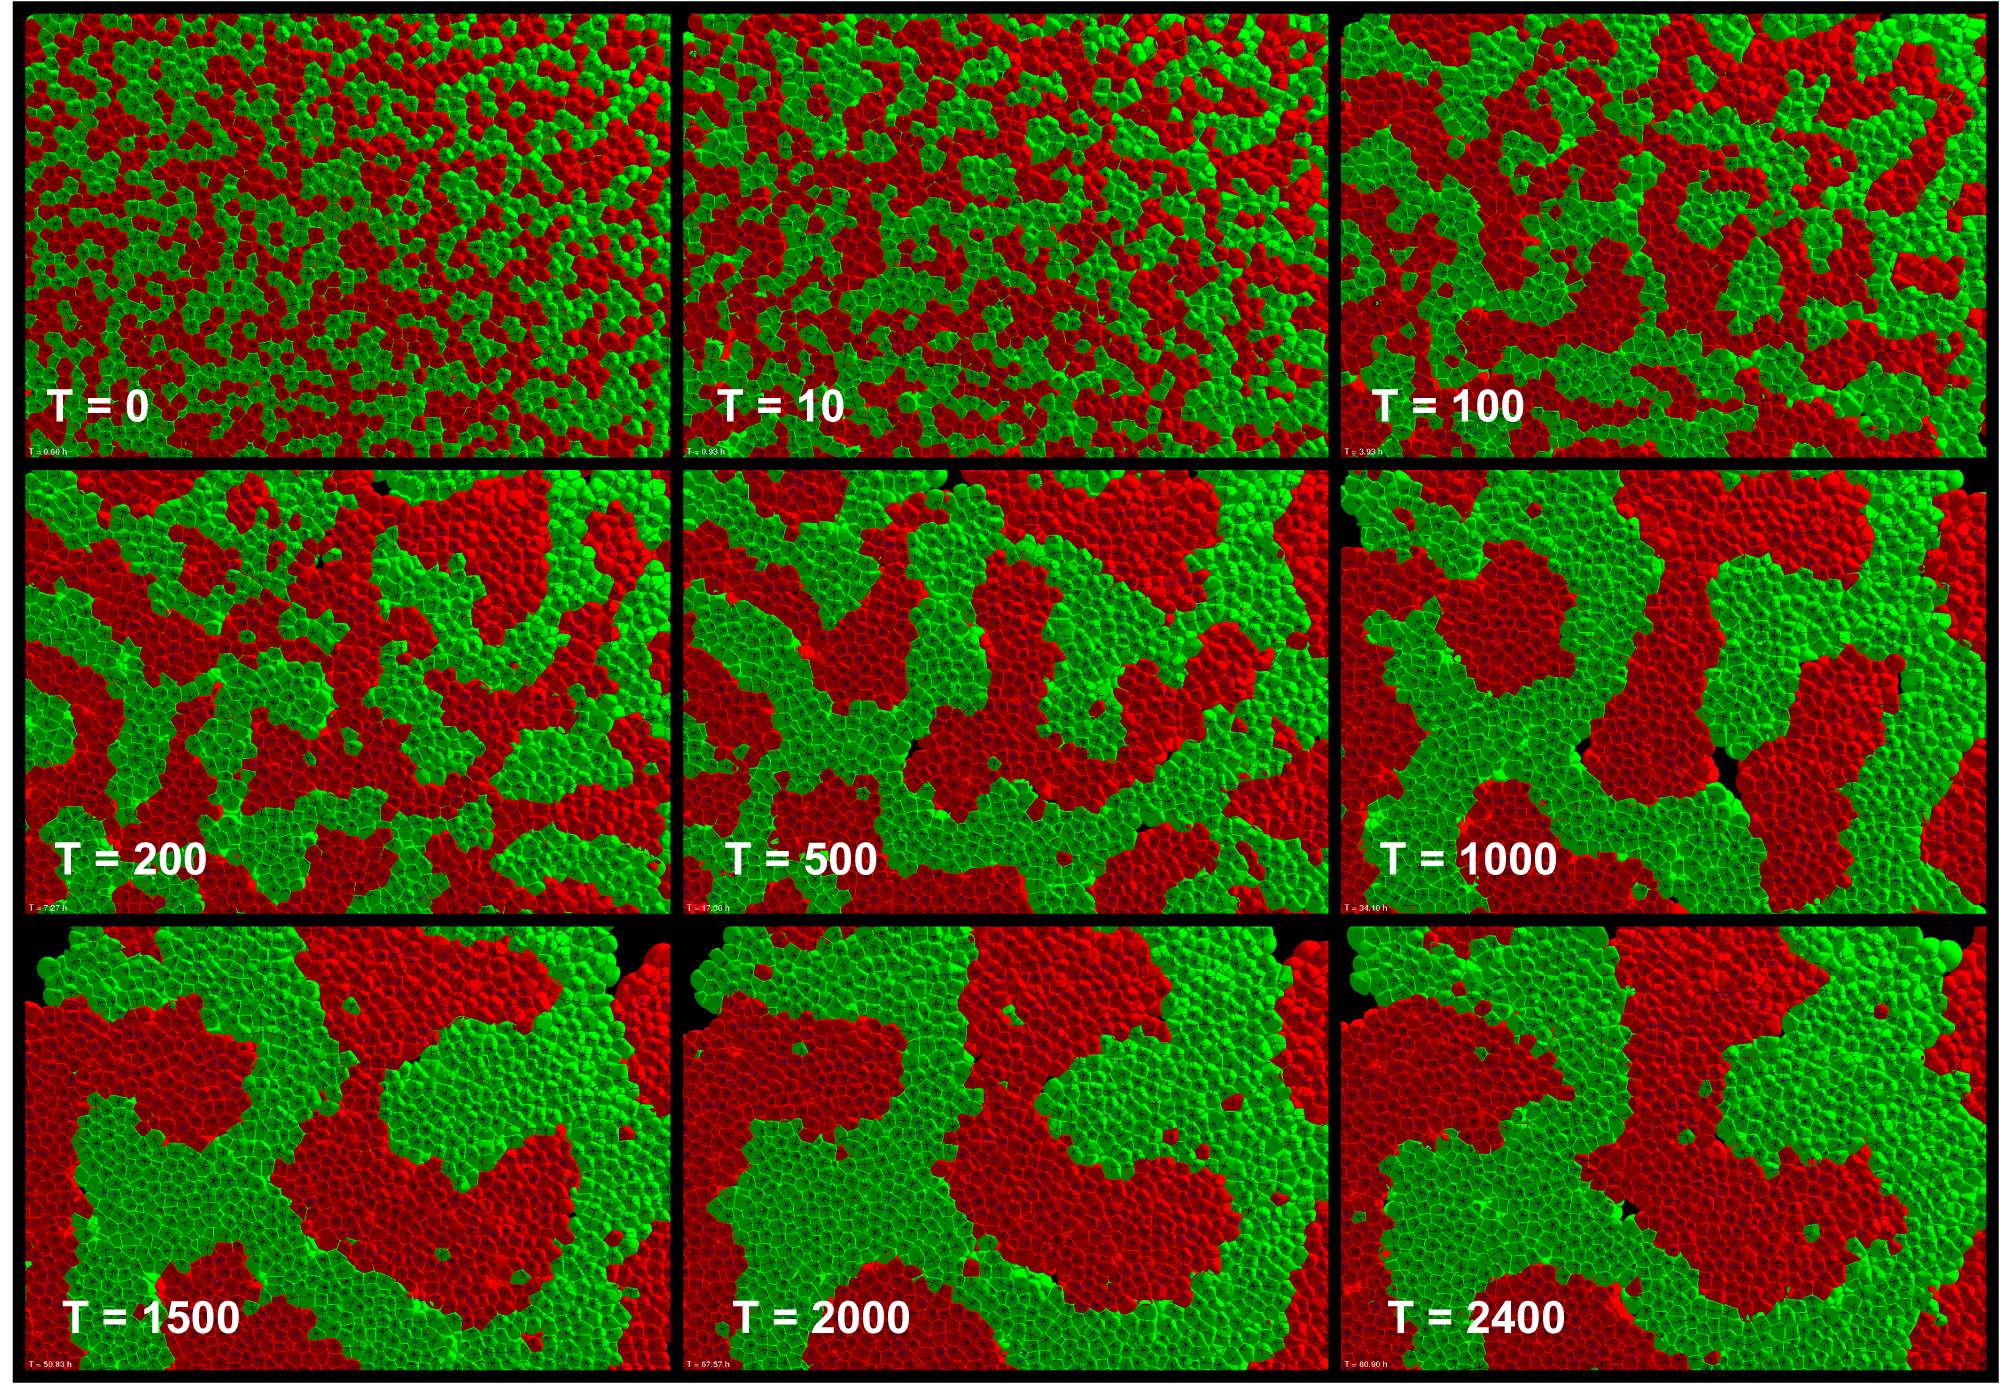
\includegraphics[width=0.9\textwidth]{../../images/Cases_Studies/Case_theo/sorting_nosource_allmigr_DAH.png}
\end{center}
\caption{\textbf{Cell sorting experiment: random axes, differential adhesion case.} The homotypic adhesion coefficient ($w_{\mathrm{adh}} = 5$) is higher than the heterotic coefficient ($w_{\mathrm{adh}} = 1$). All cells have bipolar protrusive activities with random polarization axes (mode (d) in Section 5.1). The rate of cluster size growth is decreasing over time. The time is provided through the number of simulation time steps.}
\label{Case_theo_sorting_nosource_allmigr_DAH_image}
\end{figure}


\paragraph{Oriented protrusion exterior morphogenetic field, source left right}
%  ++++++++++++++++++++++++++++++++++++++++++++++++++++++++++++++++++++++ 


  In the second experiment, the homotypic adhesion is once again stronger than the heterotypic adhesion. However, the polarization axis are not random in this case. Two different ligands are secreted from opposite border of the swarm, red cells are responding to one ligand (i.e. the left border in Fig. \ref{Case_theo_sorting_sourceext_extmigr_image}) and green cells to the other ligand (i.e. the right border in Fig. \ref{Case_theo_sorting_sourceext_extmigr_image}). Every cells adopt the local gradient-based mode of polarization ((a) in Section 5.1), so that the red (resp. green) cells orient their polarization axis toward the left (resp. right) border. The protrusive contact are in this case only heterotypic, i.e. cells exert an active protruding force only on their neighbors which belong to the other cell type. All the mechanical interactions occur at the interface between the two populations, in opposition to the first case. We observe that the border does not become flat as we would expect from a classical study of cell sorting. This is due to the forced parallelism of the polarization axes, the inclination of the border at the later time steps of the experiment (post $T=3500$ on Fig. \ref{Case_theo_sorting_sourceext_extmigr_image}) is a direct consequence of the angle which define the pole of a cell. No cell belonging to the other population is present in this polar domain and no active forces are exerted. 
\begin{figure}
\begin{center}
\includegraphics[width=0.9\textwidth]{../../images/Cases_Studies/Case_theo/sorting_sourceext_extmigr.png}
\end{center}
\caption{\textbf{Cell sorting experiment: heterotypic protrusion, parallel polarization axes case.} Two hidden ligands are diffusing from the left and right border of the cellular bilayer. Green cells' polarization axes are oriented toward the right source and red cells' ones toward the left source (mode (a) in Section 5.1). For each cell types, cells are exerting monoplar protrusion on the other cell type only (heterotypic protrusion contacts). Heterotypic adhesion is weak ($w_{\mathrm{adh}} = 0.1$) compared to homotypic adhesion ($w_{\mathrm{adh}} = 1$). }
\label{Case_theo_sorting_sourceext_extmigr_image}
\end{figure}


\paragraph{Oriented protrusion exterior morphogenetic field, source center}
%  ++++++++++++++++++++++++++++++++++++++++++++++++++++++++++++++++++++++ 


  The third experiment is similar as the second one, strong homotypic adhesion, weak heterotypic adhesion, but a single ligand is secreted from the center of the swarm. Red cells orient their polarization axes toward the source of the ligand (positive local gradient) and the green cells in the opposite direction (negative local gradient). Similarly to the previous experiment and for the same reason, the border between red and green cell population is no smooth (Fig. \ref{Case_theo_sorting_sourcecenter_extmigr_image}). 
\begin{figure}
\begin{center}
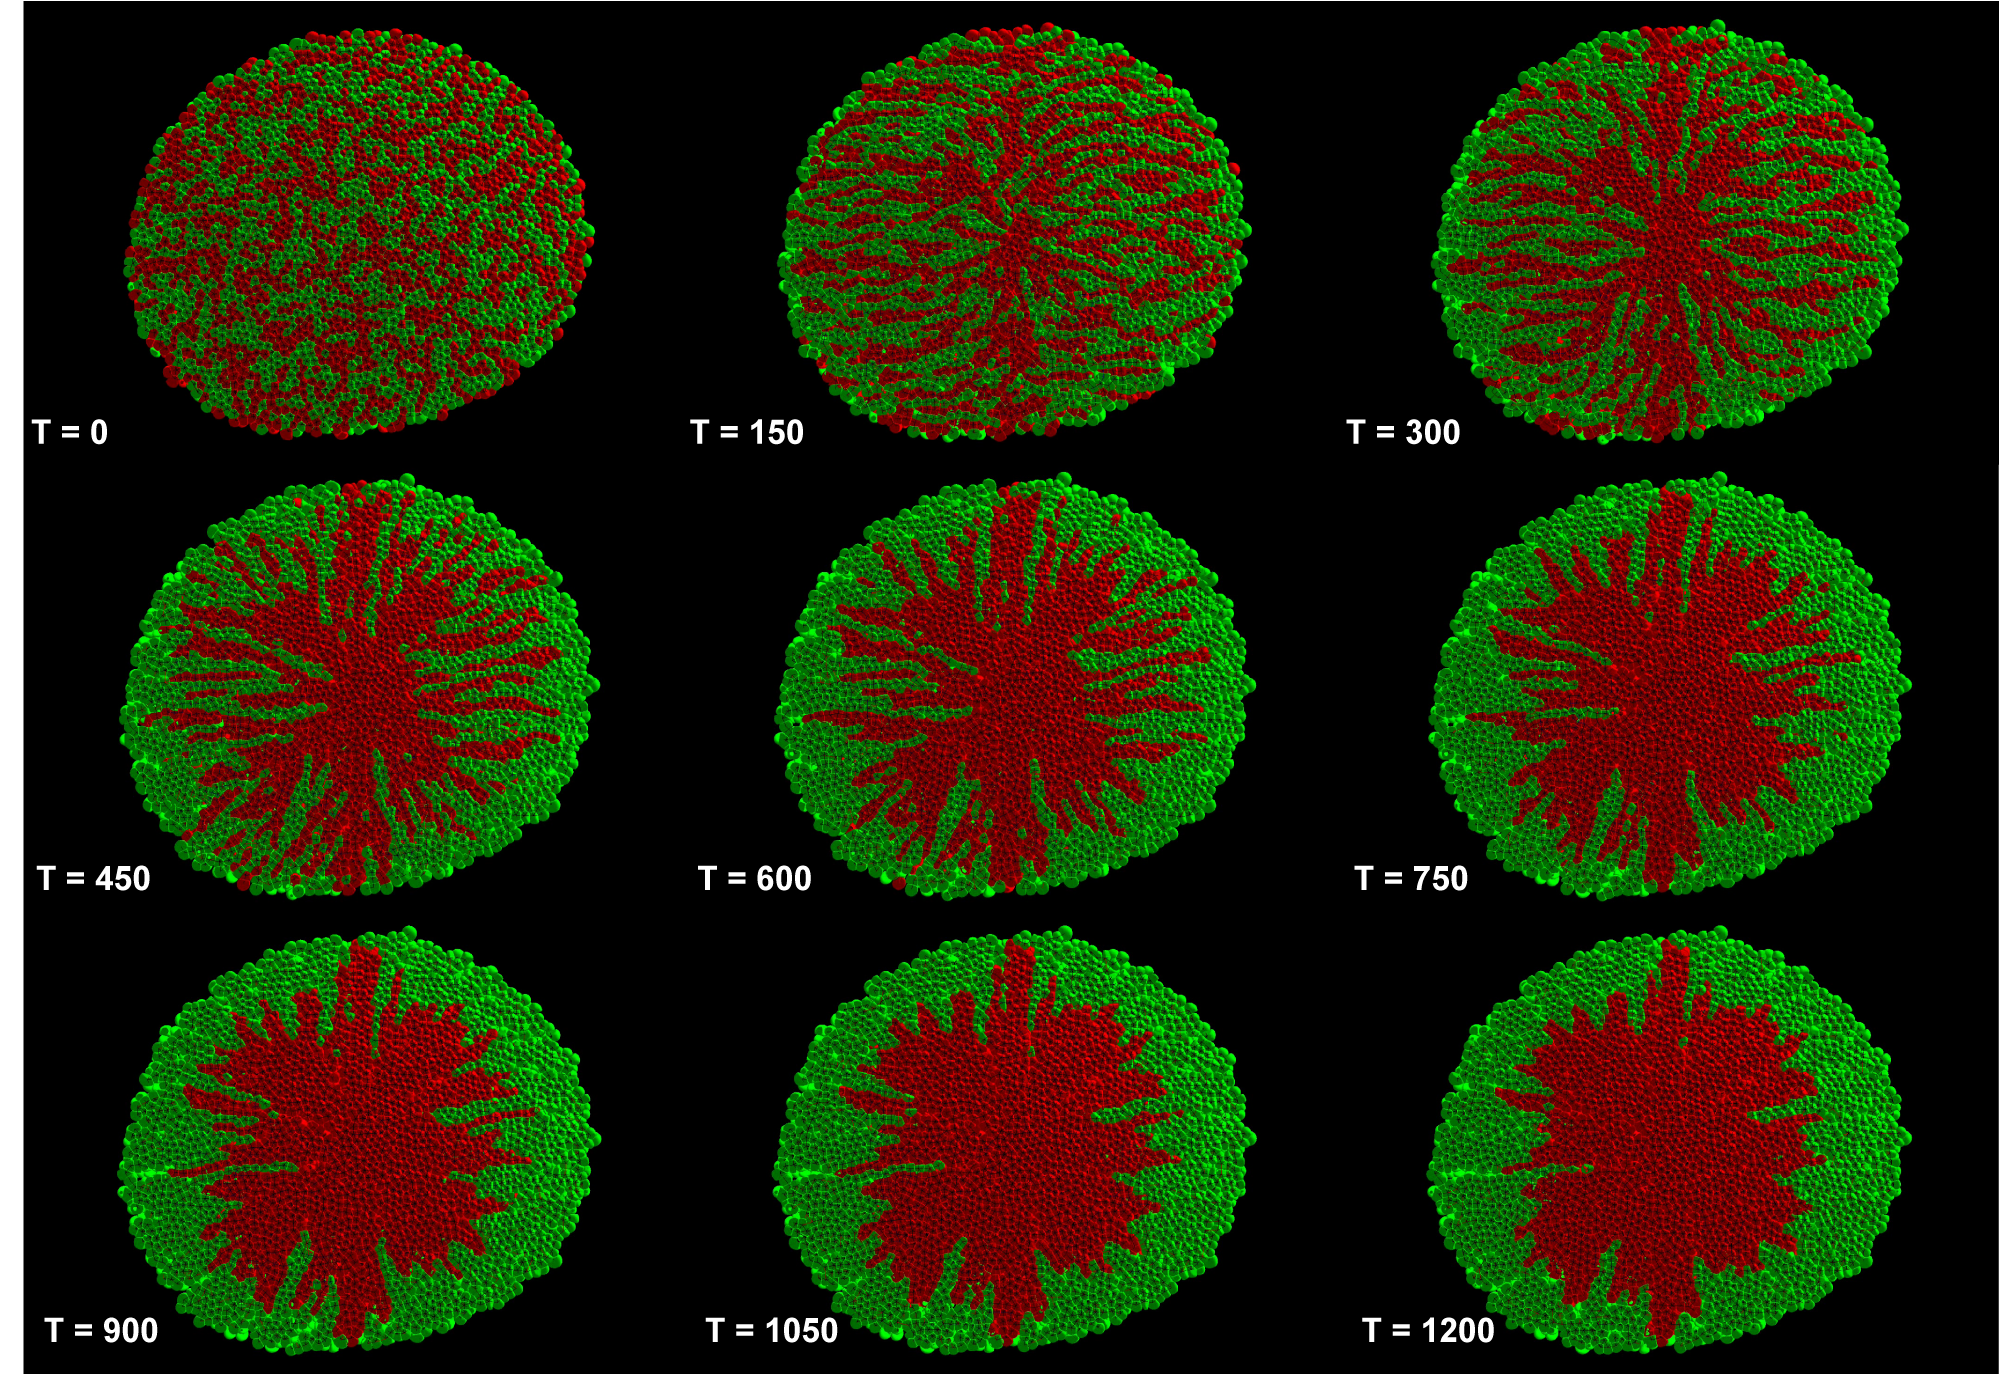
\includegraphics[width=0.9\textwidth]{../../images/Cases_Studies/Case_theo/sorting_sourcecenter_extmigr.png}
\end{center}
\caption{\textbf{Cell sorting experiment: heterotypic protrusion, radial polarization axes case.} A single ligand is diffusing from the center of the cellular bilayer. Red cells' polarization axes are oriented along the local increasing gradient, green cells' ones are oriented the local decreasing gradient (mode (a) in Section 5.1). For each cell types, cells are exerting monopolar protrusion on the other cell type only (heterotypic protrusion contacts). Heterotypic adhesion is weak ($w_{\mathrm{adh}} = 0.1$) compared to homotypic adhesion ($w_{\mathrm{adh}} = 1$).}
\label{Case_theo_sorting_sourcecenter_extmigr_image}
\end{figure}

%  ---------------------------------------------------------------------- 


\subsubsection{Single Cell Migration}
%  ---------------------------------------------------------------------- 


  This experiment is an example of the generality of the protrusive behavior in MECAGEN. The parameter involved in this study are the same as for the sorting experiment, i.e. the adhesion coefficient $w_{\mathrm{adh}}$ and protrusive force parameters. We developed a simple scenario to qualitatively mimic the migrating behavior of the germ cells observed in zebrafish embryos by the E. Raz Lab (Fig. \ref{Case_theo_individual_migration2}). Three population are involved: a population of packed cells secreting a ligand, a vast majority of inactive cells and a few migrating cells which are attracted by the ligand. The migrating cells are orienting their polarization axis through the local-gradient-based mode and exert monopolar protruding activity of their neighbors. The parameters of the relaxation forces are the same for all cells of the experiment. We observe that the simulated cells (Movie \href{http://public.iscpif.fr/~delile/morphogenesis/manuscript/pragma/figure.html?name=Case_theo_migr_raz_simu}{.5.4}) behave in a similar fashion as the real ones imaged by the E. Raz Lab (Movie \href{http://public.iscpif.fr/~delile/morphogenesis/manuscript/pragma/figure.html?name=Case_theo_migr_raz_live}{.5.5}). 
\begin{figure}
\begin{center}
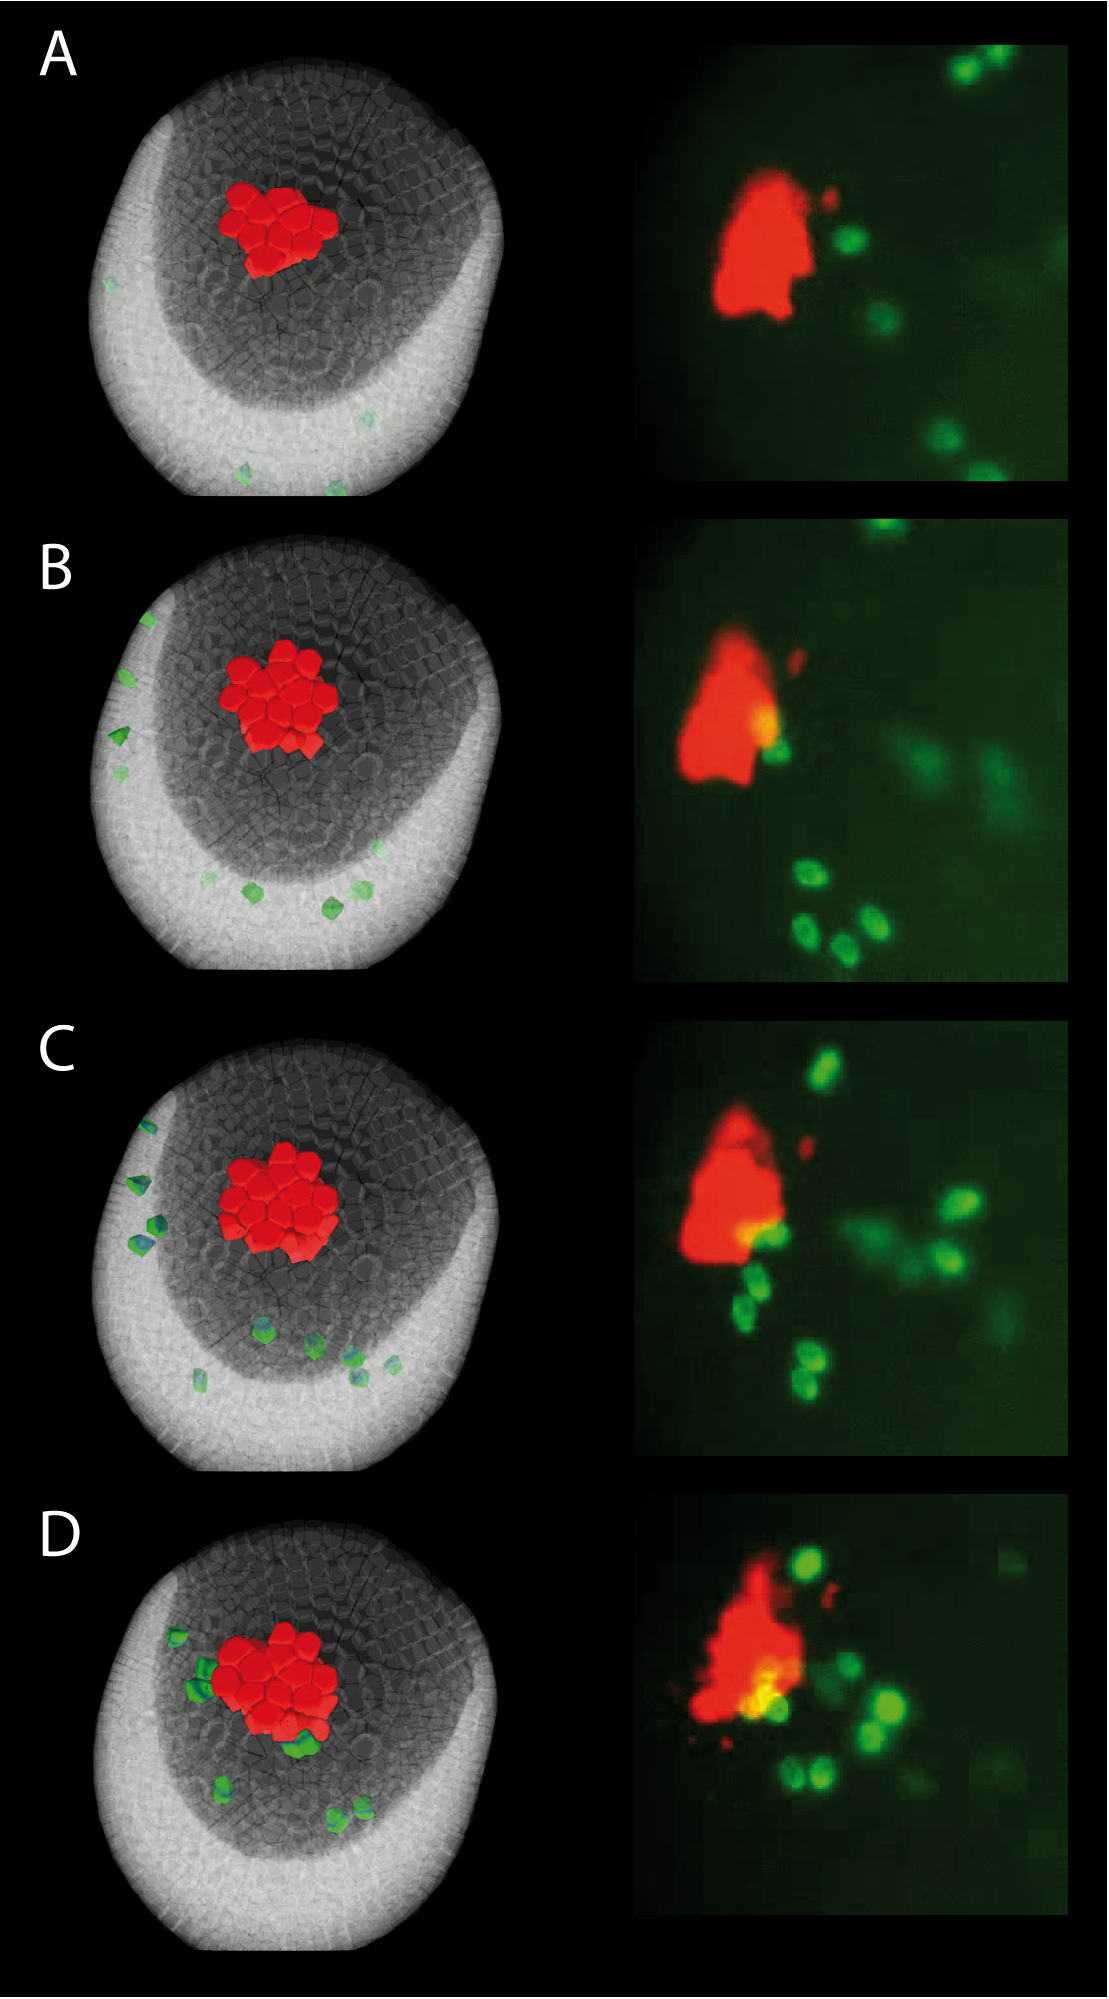
\includegraphics[width=0.5\textwidth]{../../images/Cases_Studies/Case_theo/individual_migration2.png}
\end{center}
\caption{\textbf{Cell migration experiment: individual migration. } Left: Simulation involving a three cell population: a few cells secrete a ligand (the cells are not shown but the red color represents the ligand around cells whether its local quantity is larger than a given threshold), the green cells are exerting monopolar protrusion oriented along the positive local gradient of the gradient. The protrusions are effective on every other cell types. Transparent cells are inactive. Right: Germ cells (green) migrating toward cells expressing SDF-1a (red), which serves as a guidance cue. Images from the right column adapted from a movie available on the E. Raz Lab's website http://zmbe.uni-muenster.de/institutes/izb/izbres.htm}
\label{Case_theo_individual_migration2}
\end{figure}


